\documentclass[letterpaper]{article}
\usepackage[margin=1in]{geometry}
\usepackage[utf8]{inputenc}
\usepackage{textcomp}
\usepackage{amssymb}
\usepackage{natbib}
\usepackage{graphicx}
\usepackage{gensymb}
\usepackage{amsthm, amsmath, mathtools}
\usepackage[dvipsnames]{xcolor}
\usepackage{enumerate}
\usepackage{mdframed}
\usepackage[most]{tcolorbox}
\usepackage{csquotes}
% https://tex.stackexchange.com/questions/13506/how-to-continue-the-framed-text-box-on-multiple-pages

\tcbuselibrary{theorems}

\newcommand{\R}{\mathbb{R}}
\newcommand{\Z}{\mathbb{Z}}
\newcommand{\N}{\mathbb{N}}
\newcommand{\Q}{\mathbb{Q}}
\newcommand{\C}{\mathbb{C}}
\newcommand{\code}[1]{\texttt{#1}}
\newcommand{\mdiamond}{$\diamondsuit$}
\newcommand{\PowerSet}{\mathcal{P}}
\newcommand{\Mod}[1]{\ (\mathrm{mod}\ #1)}
\DeclareMathOperator{\lcm}{lcm}

%\newtheorem*{theorem}{Theorem}
%\newtheorem*{definition}{Definition}
%\newtheorem*{corollary}{Corollary}
%\newtheorem*{lemma}{Lemma}
\newtheorem*{proposition}{Proposition}


\newtcbtheorem[number within=section]{theorem}{Theorem}
{colback=green!5,colframe=green!35!black,fonttitle=\bfseries}{th}

\newtcbtheorem[number within=section]{definition}{Definition}
{colback=blue!5,colframe=blue!35!black,fonttitle=\bfseries}{def}

\newtcbtheorem[number within=section]{corollary}{Corollary}
{colback=yellow!5,colframe=yellow!35!black,fonttitle=\bfseries}{cor}

\newtcbtheorem[number within=section]{lemma}{Lemma}
{colback=red!5,colframe=red!35!black,fonttitle=\bfseries}{lem}

\newtcbtheorem[number within=section]{example}{Example}
{colback=white!5,colframe=white!35!black,fonttitle=\bfseries}{def}

\newtcbtheorem[number within=section]{note}{Important Note}{
        enhanced,
        sharp corners,
        attach boxed title to top left={
            xshift=-1mm,
            yshift=-5mm,
            yshifttext=-1mm
        },
        top=1.5em,
        colback=white,
        colframe=black,
        fonttitle=\bfseries,
        boxed title style={
            sharp corners,
            size=small,
            colback=red!75!black,
            colframe=red!75!black,
        } 
    }{impnote}
\usepackage[utf8]{inputenc}
\usepackage[english]{babel}
\usepackage{fancyhdr}
\usepackage[hidelinks]{hyperref}

\pagestyle{fancy}
\fancyhf{}
\rhead{Math 170A}
\chead{Wednesday, January 11, 2023}
\lhead{Lecture 2}
\rfoot{\thepage}

\setlength{\parindent}{0pt}

\newcommand{\mb}{\mathbf{b}}
\newcommand{\mx}{\mathbf{x}}

\begin{document}
\section{Systems of Linear Equations (Section 1.2)}
This section is mainly going to be reviewing systems of linear equations.

\subsection{Nonsingularity and Uniqueness of Solutions}
Suppose we have a system of $n$ linear equations and $n$ unknowns
\begin{equation} \label{1-14:1}
    \begin{split}
        a_{11}x_1 + a_{12}x_2 + &\hdots + a_{1n}x_n = b_1 \\
        a_{21}x_1 + a_{22}x_2 + &\hdots + a_{2n}x_n = b_2 \\
        &\vdots \\
        a_{n1}x_1 + a_{n2}x_2 + &\hdots + a_{nn}x_n = b_n.
    \end{split}
\end{equation}
We're given the coefficients $a_{ij}$ and $b_i$, and we want to find $x_1, \hdots, x_n$ that satisfies the equations. Generally, it's tedious to write (\ref{1-14:1}) over and over again, so we might write it as a single matrix equation 
\begin{equation} \label{1-14:2}
    A\mx = \mb,
\end{equation}
where 
\[A = \begin{bmatrix}
    a_{11} & a_{12} & \hdots & a_{1n} \\ 
    a_{21} & a_{22} & \hdots & a_{2n} \\ 
    \vdots & \vdots &        & \vdots \\ 
    a_{n1} & a_{n2} & \hdots & a_{nn}
\end{bmatrix} \quad \mx = \begin{bmatrix}
    x_1 \\ x_2 \\ \vdots \\ x_n
\end{bmatrix} \quad \mb = \begin{bmatrix}
    b_1 \\ b_2 \\ \vdots \\ b_n
\end{bmatrix}.\]
In other words, we are given $A$ and $\mb$ and must solve for $\mx$. $A \in \R^{n \times n}$ is an $n \times n$ matrix, also known as a \emph{square matrix}.

\bigskip 

Note that (\ref{1-14:2}) has a unique solution if and only if the matrix $A$ is nonsingular. 

\begin{theorem}{}{1-14:3}
    Let $A$ be a square matrix. The following six conditions are equivalent; that is, if any one holds, they all hold: 
    \begin{enumerate}[(a)]
        \item $A^{-1}$ exists. 
        \item There is no nonzero $\mathbf{y}$ such that $A\mathbf{y} = \mathbf{0}$.
        \item The columns of $A$ are linearly independent.
        \item The rows of $A$ are linearly independent. 
        \item $\det(A) \neq 0$.
        \item Given any vector $b$, there is exactly one vector $\mx$ such that $A\mx = \mb$. 
    \end{enumerate}
\end{theorem}
\textbf{Remark:} Existence and uniqueness of $\mx$ only depends on $A$ and not on $\mb$.

To briefly review the inverse of a matrix, we should note that the $n \times n$ \textbf{identity matrix} is denoted by $I$, and is the unique matrix such that 
\[AI = IA = A\]
for all $A \in \R^{n \times x}$.The identity matrix has \code{1}'s on its main diagonal and \code{0}'s everywhere else. For example, the $3 \times 3$ identity matrix has the form 
\[I = \begin{bmatrix}
    1 & 0 & 0 \\ 
    0 & 1 & 0 \\ 
    0 & 0 & 1
\end{bmatrix}.\]
Given a matrix $A$, if there is a matrix $B$ such that $AB = BA = I$, the $B$ is called the inverse of $A$ and is denoted $A^{-1}$. \emph{Not every matrix will have an inverse.}

\bigskip 

In any case, if the conditions of Theorem \ref{th:1-14:3} hold, $A$ is said to be nonsingular or invertible. If the conditions do \emph{not} hold, then $A$ is said to be singular or noninvertible. In this case, \ref{1-14:2} will have no solution or infinitely many solutions. 

\bigskip 

Now, we'll focus on when $A$ is nonsingular. In this case, the unique solution of \ref{1-14:2} can be obtained by multiplying both sides by $A^{-1}$. We can see this from how 
\begin{equation*}
    \begin{aligned}
        A\mx &= \mb \\ 
            &\implies A^{-1} A \mx = A^{-1} \mb \\ 
            &\implies I\mx = A^{-1}\mb \\ 
            &\implies \mx = A^{-1}\mb. 
    \end{aligned}
\end{equation*}
While this is guaranteed to solve the problem, doing so is a bad idea as it's very error-prone. It's usually a better idea to solve $A\mx = \mb$. It should also be noted that computing $A^{-1}$ is computationally expensive.

\bigskip 

\textbf{Note:} We can use MATLAB to solve for $\mx$ by using 
\begin{verbatim}
    x = A \ b\end{verbatim}

\subsection{Numerical (Approximate) Solution of Differential Equations}
In this section, we'll focus on ordinary differential equations (ODE). These contain one or more functions of one independent variable and the derivatives of those functions. For example, consider the initial value system 
\begin{equation}\label{1-14:4}
    \begin{cases}
        u'(x) + au(x) = f(x) \\ 
        u(0) = 0
    \end{cases}
\end{equation}
with $x \in [0, 1]$. We have two functions, $f(x)$ and $u(x)$, derivative $u'(x)$, and one independent variable $x$. Suppose a fixed $a \in \R$ and $f: \R \mapsto \R$. Our goal is to find a function $u$ satisfying the system (\ref{1-14:4}).

\begin{enumerate}
    \item First, approximate $u'$. 
    \[u'(x) = \lim_{h \mapsto 0} \frac{u(x + h) - u(x)}{h} = \lim_{h \mapsto 0} \frac{u(x) - u(x - h)}{h} = \lim_{h \mapsto 0} \frac{u(x + h) - u(x - h)}{2h}.\]
    We want to pick a very small $h$ to do this evaluation. That way, for a small enough $h$ (close to 0), we can do 
    \begin{equation}\label{1-14:5}
        u'(x) \approx \frac{u(x + h) - u(x)}{h} \approx \frac{u(x) - u(x - h)}{h} \approx \frac{u(x + h) - u(x - h)}{2h}
    \end{equation}

    \item To choose a small $h$, we can divide the given interval, which in this case is $[0, 1]$, into $m$ subintervals. Pick a (possibly large) $m \in \N$, and then subdivide the interval into $m$ equal subintervals of length $h = \frac{1}{m}$. 
    
    \begin{center}
        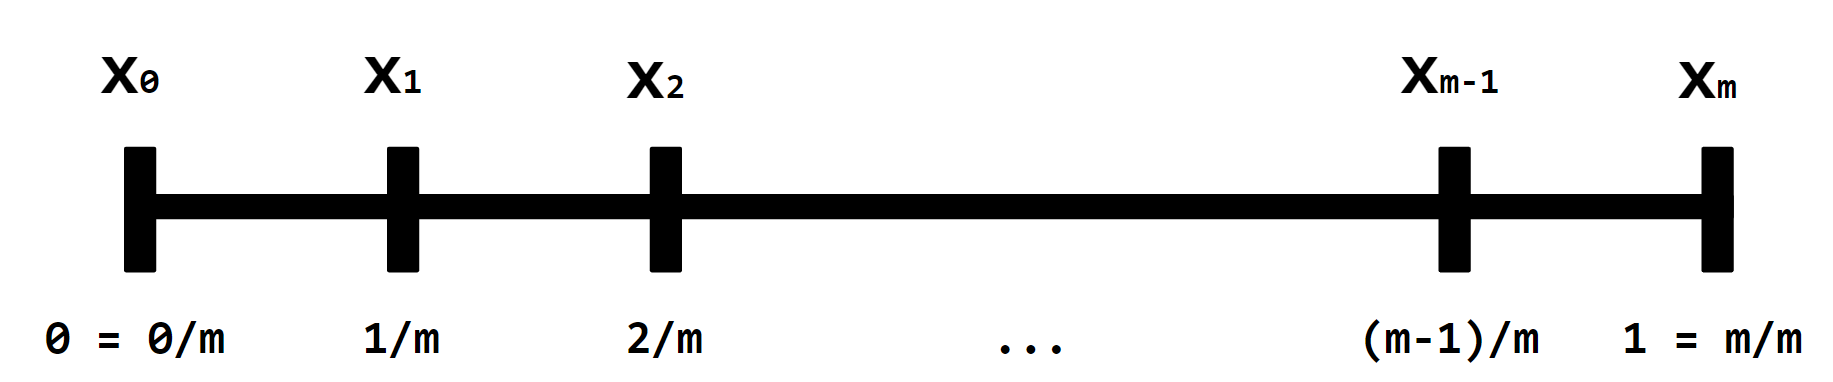
\includegraphics[scale=0.4]{../assets/sub_divide.png}
    \end{center}
    
    The subdivision points of the intervals would be $x_i = \frac{i}{m}$ for $i = 0, 1, 2, \hdots, m$. That way, we can find $u$ on those points; that is, we can find \[u\left(x_i = \frac{i}{m}\right).\] 
    With this in mind, the approximation formula from (\ref{1-14:5}) can be rewritten as such:
    \[u'(x_i) \approx \frac{u(x_i + h) - u(x_i)}{h} \approx \frac{u(x_i) - u(x_i - h)}{h} \approx \frac{u(x_i + h) - u(x_i - h)}{2h},\]
    or just 
    \[u'(x_i) \approx \frac{u(x_{i + 1}) - u(x_{i})}{h} \approx \frac{u(x_i) - u(x_{i - 1})}{h} \approx \frac{u(x_{i + 1}) - u(x_{i - 1})}{2h}.\] 
    The approximation used depends on the information you are given.
    \item Now, we can set up a linear system. We want to find $u(x_i)$ for all $i \in [0, m]$. 
    \begin{itemize}
        \item For $i = 0$, it's clear that 
        \[u(x_i) = u(x_0) = u(0) = 0\]
        from the given condition.

        \item For $i = 1$, we can use the approximation 
        \[u'(x_i) \approx \frac{u(x_i) - u(x_{i - 1})}{h}\]
        to get 
        \begin{equation*}
            \begin{aligned}
                &\frac{u(x_1) - u(x_0)}{h} + au(x_1) = f(x_1) \\ 
                    &\implies \frac{u(x_1) - u(0)}{\frac{1}{m}} + au(x_1) = f(x_1) \\ 
                    &\implies mu(x_1) + au(x_1) = f(x_1) \\ 
                    &\implies mu\left(\frac{1}{m}\right) + au\left(\frac{1}{m}\right) = f\left(\frac{1}{m}\right) \\ 
                    &\implies u\left(\frac{1}{m}\right) (m + a) = f\left(\frac{1}{m}\right) \\ 
                    &\implies u\left(\frac{1}{m}\right) = \frac{f\left(\frac{1}{m}\right)}{m + a}
            \end{aligned}
        \end{equation*}

        \item For $i = 2$, we can use the approximation
        \[u'(x_i) \approx \frac{u(x_i) - u(x_{i - 1})}{h}\]
        to get 
        \begin{equation*}
            \begin{aligned}
                &\frac{u(x_2) - u(x_1)}{h} + au(x_2) = f(x_2) \\ 
                    &\implies \frac{u(x_2) - u(x_1)}{\frac{1}{m}} + au(x_2) = f(x_2) \\ 
                    &\implies m\left(u(x_2) - u(x_1)\right) + au(x_2) = f(x_2) \\ 
                    &\implies mu(x_2) - mu(x_1) + au(x_2) = f(x_2) \\ 
                    &\implies u(x_2)(m + a) - mu(x_1) = f(x_2) \\ 
                    &\implies u(x_2)(m + a) = mu(x_1) + f(x_2) \\ 
                    &\implies u(x_2) = \frac{mu(x_1) + f(x_2)}{m + a} \\ 
                    &\implies u\left(\frac{2}{m}\right) = \frac{mu\left(\frac{1}{m}\right) + f\left(\frac{2}{m}\right)}{m + a}.
            \end{aligned}
        \end{equation*}
        Note that we found $u\left(\frac{1}{m}\right)$ in the previous step.

        \item For $i = m$, we have 
        \begin{equation*}
            \begin{aligned}
                &\frac{u(x_m) - u(x_{m - 1})}{h} + au(x_m) = f(x_m) \\ 
                    &\implies \frac{u(1) - u(x_{m - 1})}{\frac{1}{m}} + au(1) = f(1) \\ 
                    &\implies m(u(1) - u(x_{m - 1})) + au(1) = f(1) \\ 
                    &\implies mu(1) - mu(x_{m - 1}) + au(1) = f(1) \\ 
                    &\implies u(1)(m + a) - mu(x_{m - 1}) = f(1) \\ 
                    &\implies u(1)(m + a) = mu(x_{m - 1}) + f(1) \\ 
                    &\implies u(1) = \frac{mu(x_{m - 1}) + f(1)}{m + a} \\ 
                    &\implies u(1) = \frac{mu(\frac{m - 1}{m}) + f(1)}{m + a}.
            \end{aligned}
        \end{equation*}
    \end{itemize}
\end{enumerate}

With this all in mind, we want to be able to generate a linear system of the form 
\begin{equation*}
    \begin{aligned}
        &\begin{cases}
            u\left(\frac{1}{m}\right) = \frac{f\left(\frac{1}{m}\right)}{m + a} \\ 
            u\left(\frac{2}{m}\right) = \frac{mu\left(\frac{1}{m}\right) + f\left(\frac{2}{m}\right)}{m + a} \\ 
            \vdots \\ 
            u(1) = \frac{mu(\frac{m - 1}{m}) + f(1)}{m + a}
        \end{cases} \\ 
        &\implies \begin{cases}
            (m + a) u\left(\frac{1}{m}\right) = f\left(\frac{1}{m}\right) \\ 
            (m + a) u\left(\frac{2}{m}\right) = mu\left(\frac{1}{m}\right) + f\left(\frac{2}{m}\right) \\ 
            \vdots \\ 
            (m + a) u(1) = mu(\frac{m - 1}{m}) + f(1)
        \end{cases} \\ 
        &\implies \begin{cases}
            (m + a) u\left(\frac{1}{m}\right) = f\left(\frac{1}{m}\right) \\ 
            -mu\left(\frac{1}{m}\right) + (m + a) u\left(\frac{2}{m}\right) = f\left(\frac{2}{m}\right) \\ 
            \vdots \\ 
            -mu(\frac{m - 1}{m}) + (m + a) u(1) = f(1)
        \end{cases}.
    \end{aligned}
\end{equation*}
Representing it with matrices, we have 
\begin{equation*}
    \begin{aligned}
        \begin{bmatrix}
            m + a & 0 & 0 & \hdots & 0 \\ 
            -m & m + a & 0 & \hdots & 0 \\ 
            0 & -m & m + a & \hdots & 0 \\ 
            \vdots & \vdots & \vdots & & \vdots \\ 
            0 & 0 & 0 & \hdots & m + a
        \end{bmatrix} \begin{bmatrix}
            u(x_1) \\ u(x_2) \\ u(x_3) \\ \vdots \\ u(x_m)
        \end{bmatrix} = \begin{bmatrix}
            f\left(\frac{1}{m}\right) \\ 
            f\left(\frac{2}{m}\right) \\ 
            f\left(\frac{3}{m}\right) \\ 
            \vdots \\ 
            f\left(\frac{m}{m}\right)
        \end{bmatrix}.
    \end{aligned}
\end{equation*}
\textbf{Remarks:}
\begin{itemize}
    \item Note that if you choose a different approximation, you will get a different left-hand and right-hand side.
    \item A larger $m$ gives a better approximation, but the resulting linear system is larger as well. 
\end{itemize}
Ultimately, the goal here is to solve the linear system $A\mx = \mb$ to find $u(x_1), u(x_2), \hdots, u(x_m)$. This is the approximation to $u$.

\subsection{Solving Diagonal Systems}
Let's start with the simplest kind of linear system to solve.
\[\begin{bmatrix}
    a_{11} & 0 & 0 & \hdots & 0 \\ 
    0 & a_{22} & 0 & \hdots & 0 \\ 
    0 & 0 & a_{33} & \hdots & 0 \\ 
    \vdots & \vdots & \vdots & & \vdots  \\ 
    0 & 0 & 0 & \hdots & a_{nn}
\end{bmatrix} \begin{bmatrix}
    x_1 \\ x_2 \\ x_3 \\ \vdots \\ x_n
\end{bmatrix} = \begin{bmatrix}
    b_1 \\ b_2 \\ b_3 \\ \vdots \\ b_n
\end{bmatrix}.\]
Writing this as a system of linear equations gives 
\[\begin{cases}
    a_{11}x_1 + 0x_2 + \hdots + 0x_n = b_1 \\ 
    0x_1 + a_{22}x_2 + \hdots + 0x_n = b_2 \\ 
    \vdots \\ 
    0x_1 + 0x_2 + \hdots + a_{nn}x_n = b_n 
\end{cases} \implies \begin{cases}
    a_{11}x_1 = b_1 \\ 
    a_{22}x_2 = b_2 \\ 
    \vdots \\ 
    a_{nn}x_n = b_n 
\end{cases}.\]
The solution is just 
\[x_1 = \frac{b_1}{a_{11}} \qquad x_2 = \frac{b_2}{a_{22}} \qquad \hdots \qquad x_n = \frac{b_n}{a_{nn}}.\]
We can write an algorithm to solve this as well. 
\begin{algorithmic}
    \State $\mx \gets \mathbf{0}$
    \For{$i = 1, \hdots, n$}
        \State $x_i \gets \frac{\mb_i}{A_{ii}}$
    \EndFor
\end{algorithmic}
From this, it follows that the flop count is just $n$, and its Big-O is $\BigO(n)$. 

\end{document}